\documentclass[12pt,a4paper]{report}
\usepackage[utf8]{inputenc}
\usepackage{amsmath}
\usepackage{amsfonts}
\usepackage{amssymb}
\usepackage{graphicx}
\usepackage{booktabs}
\usepackage{algorithm}
\usepackage{algpseudocode}
\usepackage{subcaption}
\usepackage[english]{babel}
\usepackage[export]{adjustbox}
\usepackage{enumerate}
\usepackage[left=3.5cm,right=2.5cm,top=2.5cm,bottom=2.5cm]{geometry}
\usepackage{lineno}
\usepackage{cite}
\usepackage{acronym}
\usepackage{url}
\renewcommand{\baselinestretch}{1.5}



\begin{document}

	\begin{center}
		\begin{LARGE}			\bf{Adaptive Multimodal Biometric Management Algorithm}
		\end{LARGE}
		\vspace*{30pt}
		
		\textbf{}
		\vspace{20pt}
		\textbf{Master of Technology\\}
		\vspace{3pt}
		{COMPUTER SCIENCE AND INFORMATION SECURITY}\\
		\vspace{40pt}
		
		\textbf{
			  NENAVATH KOMAL KESAV (25CSM2R11)\\
			  MADABHUSHI SRIKANTH (25CSM2R22)\\
			SANGIREDDY VEERA INDRASENA REDDY (25CSM2S08)}\\
		\vspace{30pt}
		
\includegraphics[width=0.3\textwidth]{./logo.png} \\
		\vspace{30pt}
		\textit{Under the guidance of}\\
		\textbf{PROF. MANISH KUMAR BAJPAI}\\
		\textit{\textbf{ASSOCIATE PROFESSOR}}
		
		
		\vspace{20pt}
		
		
		\textbf{DEPARTMENT OF COMPUTER SCIENCE AND ENGINEERING\\
			NATIONAL INSTITUTE OF TECHNOLOGY WARANGAL\\
			November, 2025
		}
	\end{center}
\pagenumbering{gobble}

\newpage
\section{Abstract}
The conventional unimodal biometric methods can be characterized as having poor accuracy and robustness because of changes in illumination, pose, and environmental factors. Currently used multimodal fusion techniques, especially those on the decision and score levels uses fixed or predefined fusion rules that limit flexibility and extrapolation to real-life scenarios. To address these shortcomings, this paper suggests an adaptive multimodal biometric recognition system which combines iris and hand geometry characteristics with deep feature extraction and various fusion principles.

The proposed system utilizes the \textbf{EfficientnetB0} to extract features based on the modality and also discusses three paradigms of fusion, including: Weighted Feature Fusion, Concatenation Fusion and Cross-Attention-based Fusion to determine which fusion mechanism is most effective in identity recognition. The cross-attention fusion process facilitates interactions between modalities, which means that the model can focus dynamically on discriminative data in modalities. The MULB multimodal biometric data is experimentally evaluated to prove that the proposed \textbf{cross-attention fusion} model delivers a better recognition performance, with the accuracy of 97.7\%, being better than that of the \textbf{concatenation-based} 96\% and \textbf{weighted fusion} 96.4\% methods.

These confirm the effectiveness of adaptive and learnable fusion strategies in multimodal biometric authentication systems to fill the current research gap between score-level and ranking fusion and emphasize the role played by attention-based deep models in subsequent biometric integration systems.

\section{Introduction}
Biometric systems based on a single modality, such as face, fingerprint, or iris, often experience considerable performance degradation under uncontrolled conditions due to noise, illumination changes, and occlusions. Unimodal systems are also prone to spoofing attacks and intra-class variations which result in the poor recognition accuracy and low reliability. To overcome these weaknesses, multimodal biometrics systems which integrate data of several physiological or behavioral characteristics have been of great interest, since they are more robust, have a better discriminative property and a greater recognition capability.

In order to address these constraints, a concept of multimodal biometric systems has been developed that integrates various types of biometric characteristics to enhance accuracy, reliability and spoofing resistance. Although multimodal approaches will considerably improve performance, new challenges are presented. The first significant difficulty is in the \textbf{heterogeneity of the spaces of features} - biometric characteristics like iris and hand geometry vary in size, dimensions and data distribution, and direct fusion is not so easy. Secondly, the \textbf{optimal fusion strategy} is another important research question, whereby the system has to decide on how to merge complementary information in each modality without redundancy and the discrimination ability of the information should not be lost. Third, multimodal systems can be challenged by issues of \textbf{computational and scalability}, particularly with large datasets and deep models in place. Finally, the ability to adapt to changing environments, such as sensor quality, lighting, or user behavior, is not easily possible in more traditional methods of fusion that are simply static.

Deep learning models have demonstrated impressive success in the last several years in the context of feature extraction and representation, in performing biometric recognition tasks. We use \textbf{EfficientNet-B0} as a deep feature extractor of iris and hand geometry modalities in this work because of the efficient use of parameters and great representative power. In order to synthesize these extracted features, three fusion mechanisms are investigated, namely feature concatenation, weighted fusion, and cross-attention-based fusion, which is executed through TensorFlow/Keras frameworks. The strategies enable us to systematically analyze the effects of each fusion strategy on the performance of multimodal biometric recognition.

There are a few attempts to improve multimodal biometric recognition considering existing literature. The initial literature used score and decision-level fusion rules and frequently based on fixed strategies like AND/OR logic or Bayesian combination models. Subsequent research proposed such evolutionary algorithm as Particle Swarm Optimization (PSO) and Ant Colony Optimization (ACO) to the adaptive selection of the rules. Even though these approaches enhanced decision-level fusion, they did not feature fine-grinned interaction in terms of features. More modern deep learning models have considered feature concatenation and attention networks, although most are still restricted to two modalities, and do not capture the so-called cross-modal dependencies that are important to complex biometric systems. Therefore, the quest to design a distinctively adaptive and computationally efficient end-to-end trainable fusion architecture has a visible gap.

The core findings of the paper are the following. To begin with, we present a suggestion of a deep multimodal biometric recognizer framework, which implies the combination of iris and hand geometry features, which are retrieved using the EfficientNet-B0. Second, we construct and test three fusion mechanisms, including concatenation, weighted fusion, and cross-attention fusion, to explore their comparative effectiveness as per the role of features integration and classification accuracy. Third, our suggested cross-attention fusion strategy is the most effective strategy as it learns fine-grained intermodal dependencies, leading to a recognition accuracy of 97.7\%, which is better than the other two strategies. Lastly, our structure fills the gap between past rule-based fusion and the present adaptive learning-based fusion by allowing the use of dynamic inter-modal feature weighting in order to improve recognition performance and system adaptability.

The rest of this article is structured in the following way. Section II is related to work and theoretical background. In Section III, the proposed methodology, such as data preprocessing, feature extraction and fusion mechanisms is described. Section IV provides the experimental results and setup. Section V brings the paper to an end, and identifies the future research directions.

\section{Related Work}
The current literature in the field of multimodal biometric authentication has been extensively explored and classified into several categories based on the fusion strategies and deep learning models adopted. Traditional unimodal biometrics systems which use only one modality such as facial recognition or fingerprint matching has turned out to have problems with sensor noise, variations in lighting and spoofing. To address these difficulties, more and more current studies have addressed multimodal systems that integrate more than one biometric feature to make them more accurate, robust, and flexible.

For instance, Zhang et al. (2022) in their work “Multimodal Feature-Level Fusion for Biometrics Identification System on IoMT Platform”, \textbf{Zhang et al. (2022)} proposed the feature level fusion model that unites multiple types of biometric characteristics (face, fingerprint, and finger vein) by using the Fisher Vector encoding and Gaussian Mixture Models (GMM). Their model had good discriminatory power and was especially successful in the case of IoMT where continuous secure authentication is needed. This paper has highlighted the importance of feature level fusion which enhances the combination of heterogeneous biometric features into one discriminatory vector to amplify recognition performance without compromising computational feasibility.

Similarly, \textbf{Li and Chen (2021)}, in Fusion to Adaptation: Investigation on Enhancing Multimodal Biometric Authentication Systems, have suggested a cross-attention based adaptive fusion mechanism which, in varying conditions of images and the environment, adjusts the weight of each modality. This deep learning-based method applied EfficientNet-B0 that is a CNN backbone at the feature extraction stage and is additionally paired with attention-guided feature weighting, which showed better results in noisy and changing conditions. Their results bring to the fore the fact that cross-attention fusion is more accurate than a mere concatenation or weighted averaging because it allows interaction and contextual alignment of feature representations.

In a comprehensive review, \textbf{Singh et al. (2023)} in the article Unimodal and Multimodal Biometric Sensing Systems: A Review gave a detailed comparison of sensor-, feature-, score-, and decision-level fusion. The authors subclassified the different fusion methods and realized that feature-level fusion has its strength of being balanced between computational and discriminative abilities, but the problem of dimensional mismatch and overfitting of deep multimodal representations are difficult to solve. It also covered how the past generations of handcrafted descriptors including the ones of PCA, Gabor filters, and many more had been supplanted with deep learning-based models like the popular ones of VGG16, ResNet, MobileNet, and EfficientNet, and how modern CNNs have transformed the processes of biometric feature extraction and representation.

In addition, in the article, \textbf{Kumar et al. (2020)} investigated the concept of a score-level fusion framework by the authors of the study, which entails the use of independent face and fingerprint modality classifiers that generate normalized scores to be combined through weighted rules in the paper, titled, Hybrid Biometric Recognition Using Score-Based Deep Feature Aggregation. This method was found to be less adaptable and unable to perform in real time compared to the mechanisms of cross-attention fusion although it was simpler to implement. The other interesting work by the authors of Gupta and Al-Maadeed (2022) was the introduction of a decision-level fusion scheme in the article titled Adaptive Ensemble Framework for Secure Biometric Verification based on deep ensemble learning that would help to increase the reliability of the system. Their model aimed at making decisions of multiple unimodal classifiers, which was greater resilience to modality failure and spoof attacks, at the expense of more computation.

Throughout these works, it is possible to identify a prominent trend, which is the tendency of contemporary multimodal biometric systems to increasingly make use of the concepts of deep learning and attention-based fusion in order to be more accurate and robust. Techniques based on feature concatenation, weighted fusion and more so cross-attention fusion, with models like EfficientNet-B0 have demonstrated higher performance because of their capacity to learn inter-modality dependencies and dynamically learn feature relevance. Nevertheless, issues like high computer cost, sensor reliance and an inadequate supply of big annotated multimodal data figures are all open research questions.

These studies combined create the basis of creating adaptive, deep-learning-based multimodal biometric systems that can provide improved performance under various conditions. The combination of attention systems and the effective feature extraction models such as EfficientNet-B0, which we have used, is a major advancement towards having the state-of-the-art accuracy, flexibility and robustness of next-generation biometric authentication.

\section{Methodology}

The proposed multimodal biometric authentication framework integrates \textbf{iris} and \textbf{hand geometry} traits to enhance identification accuracy and robustness under variable acquisition conditions. The architecture consists of four main stages: data preprocessing, feature extraction, feature fusion, and classification. The system employs \textit{EfficientNet-B0} as the deep feature extractor for both modalities, followed by three distinct fusion mechanisms---\textit{Feature Concatenation Fusion}, \textit{Weighted Fusion}, and \textit{Cross-Attention Fusion}---to generate a unified multimodal representation.

\subsection*{A. Data Preprocessing}

Let the input iris image be denoted as \( I_{iris} \) and the hand geometry image as \( I_{hand} \). Both images are resized to a fixed dimension of \(224 \times 224 \times 3\), normalized to the range \([0,1]\), and augmented using rotation, flipping, and brightness adjustments to enhance dataset diversity and generalization capability. The preprocessed inputs are then fed into the feature extraction network.

\subsection*{B. Feature Extraction}

Feature extraction for both modalities is performed using the \textit{EfficientNet-B0} model, denoted as \( F_{\theta}(\cdot) \), where \( \theta \) represents the learnable parameters of the network. The extracted feature embeddings for each modality are given by:

\begin{equation}
X_{iris} = F_{\theta}(I_{iris}), \quad X_{hand} = F_{\theta}(I_{hand})
\end{equation}

Here,
\begin{itemize}
    \item \( X_{iris} \in \mathbb{R}^{d} \): deep feature vector of the iris modality,
    \item \( X_{hand} \in \mathbb{R}^{d} \): deep feature vector of the hand geometry modality,
    \item \( d \): dimensionality of extracted features (e.g., 1280 for EfficientNet-B0).
\end{itemize}

These vectors capture distinctive textural and geometrical characteristics from each biometric source.

\subsection*{C. Fusion Mechanisms}

The extracted features \( X_{iris} \) and \( X_{hand} \) are combined using three distinct fusion strategies to evaluate performance and discriminative representation quality.

\subsubsection*{1) Feature Concatenation Fusion}

In the concatenation-based fusion approach, the feature vectors are concatenated end-to-end to form a single multimodal feature representation:

\begin{equation}
X_{concat} = [X_{iris} \, \| \, X_{hand}]
\end{equation}

where \([\,\|\,]\) denotes vector concatenation, resulting in \( X_{concat} \in \mathbb{R}^{2d} \).

The concatenated vector is then passed through a fully connected layer for nonlinear transformation:

\begin{equation}
Z_{concat} = \sigma(W_c X_{concat} + b_c)
\end{equation}

and finally classified using a softmax layer:

\begin{equation}
\hat{y} = \text{Softmax}(W_o Z_{concat} + b_o)
\end{equation}

where \( \sigma(\cdot) \) represents the ReLU activation, and \( W_c, b_c, W_o, b_o \) are trainable parameters.  
This approach is simple and efficient, though it does not explicitly model cross-modal dependencies.

\begin{figure}
    \centering
    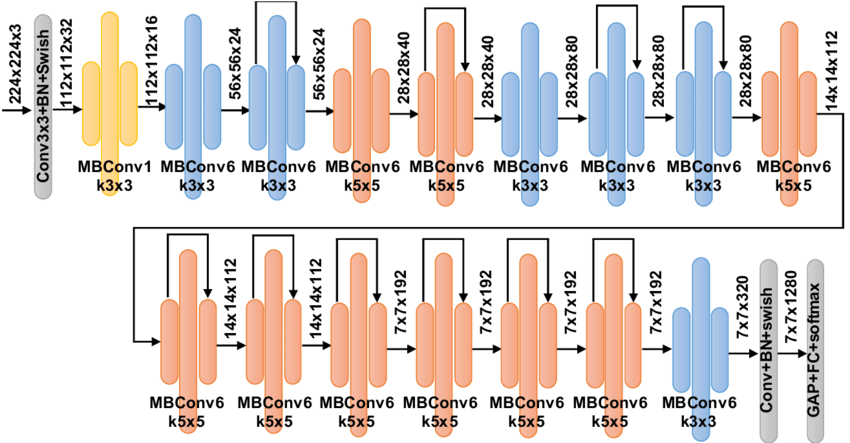
\includegraphics[width=0.7\linewidth]{The-EffecientNet-B0-general-architecture.png}
    \caption{EfficientNet-B0}
    \label{fig:placeholder}
\end{figure}

\vspace{10em}
\begin{figure}
        \centering
        
\includegraphics[width=0.8\linewidth]{image.png}
        \caption{Multimodal Biometric concatenation fusion}
        \label{fig:placeholder}
    \end{figure}

\vspace{10em}
\subsubsection*{2) Weighted Feature Fusion}

In weighted fusion, the contribution of each modality is adaptively controlled by learnable weights \( \alpha_{iris} \) and \( \alpha_{hand} \), constrained as:

\begin{equation}
\alpha_{iris} + \alpha_{hand} = 1, \quad \alpha_{iris}, \alpha_{hand} \ge 0
\end{equation}

The fused feature vector is obtained as:

\begin{equation}
X_{weighted} = \alpha_{iris} X_{iris} + \alpha_{hand} X_{hand}
\end{equation}

The weights can be dynamically learned using a softmax layer as:

\begin{equation}
[\alpha_{iris}, \alpha_{hand}] = \text{Softmax}(W_w [X_{iris} \, \| \, X_{hand}] + b_w)
\end{equation}

where \( W_w, b_w \) are learnable parameters.  
The resulting vector is transformed and classified as:

\begin{equation}
Z_{weighted} = \sigma(W_d X_{weighted} + b_d), \quad \hat{y} = \text{Softmax}(W_o Z_{weighted} + b_o)
\end{equation}

This mechanism adaptively emphasizes the modality with higher reliability, improving robustness to partial degradation.

\begin{figure}
    \centering
    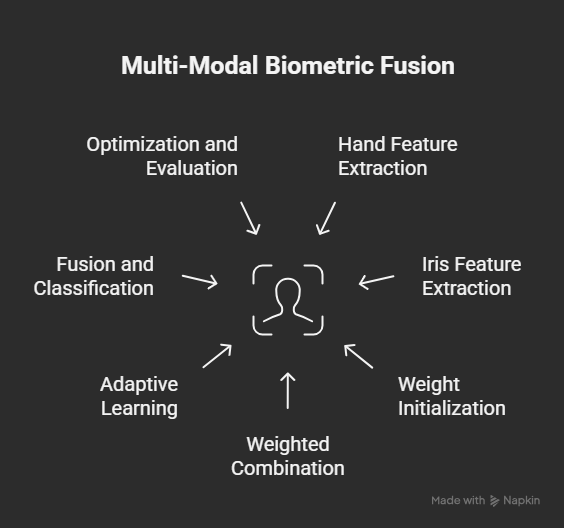
\includegraphics[width=0.7\linewidth]{_- visual selection (9).png}
    \caption{Multimodal biometric weighted fusion}
    \label{fig:placeholder}
\end{figure}

\subsubsection*{3) Cross-Attention Fusion}

The cross-attention mechanism allows each modality to learn dependencies from the other, enhancing feature interaction. Using the transformer-inspired attention operation, each modality generates queries (\(Q\)), keys (\(K\)), and values (\(V\)) as:

\begin{equation}
Q_{iris} = W_Q X_{iris}, \quad K_{hand} = W_K X_{hand}, \quad V_{hand} = W_V X_{hand}
\end{equation}

The attention from iris to hand is then computed as:

\begin{equation}
A_{iris \leftarrow hand} = \text{Softmax}\left(\frac{Q_{iris} K_{hand}^T}{\sqrt{d_k}}\right)
\end{equation}

The attended iris representation is updated as:

\begin{equation}
\tilde{X}_{iris} = A_{iris \leftarrow hand} V_{hand}
\end{equation}

Similarly, the attention from hand to iris is given by:

\begin{equation}
Q_{hand} = W_Q X_{hand}, \quad K_{iris} = W_K X_{iris}, \quad V_{iris} = W_V X_{iris}
\end{equation}

\begin{equation}
A_{hand \leftarrow iris} = \text{Softmax}\left(\frac{Q_{hand} K_{iris}^T}{\sqrt{d_k}}\right), \quad \tilde{X}_{hand} = A_{hand \leftarrow iris} V_{iris}
\end{equation}

The final cross-attended fused representation is expressed as:

\begin{equation}
X_{att} = \tilde{X}_{iris} + \tilde{X}_{hand}
\end{equation}

This feature vector is projected and classified through dense layers:

\begin{equation}
Z_{att} = \sigma(W_a X_{att} + b_a), \quad \hat{y} = \text{Softmax}(W_o Z_{att} + b_o)
\end{equation}

This mechanism captures inter-modality dependencies, focusing on complementary discriminative cues, thus yielding superior performance compared to other fusion approaches.

\begin{figure}
    \centering
    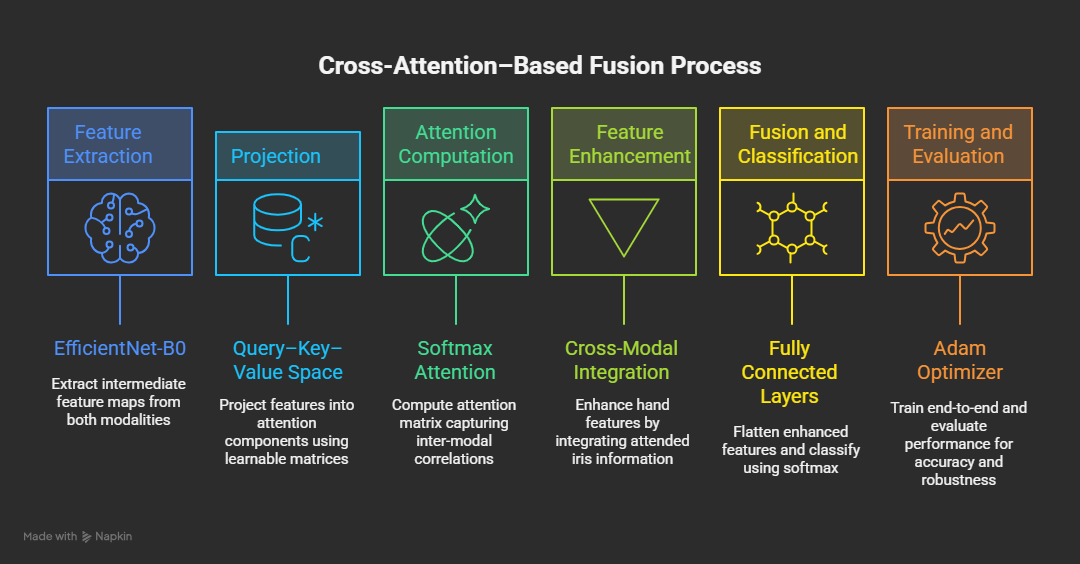
\includegraphics[width=0.8\linewidth]{Cross-Attention–Based Fusion - visual selection.png}
    \caption{Cross-Attention-Based Fusion Model}
    \label{fig:placeholder}
\end{figure}

\subsection*{D. Classification and Optimization}

The predicted output \( \hat{y} \) is compared with the ground truth label \( y \) using the categorical cross-entropy loss:

\begin{equation}
\mathcal{L} = -\sum_{i=1}^{C} y_i \log(\hat{y}_i)
\end{equation}

where \( C \) denotes the total number of identity classes. The model is optimized using the Adam optimizer with learning rate \( \eta \), and evaluated using accuracy, precision, recall, and F1-score metrics.

\subsection*{E. Summary of Fusion Techniques}

\begin{table}[h]
\centering
\caption{Comparison of Fusion Strategies}
\begin{tabular}{|p{2.5cm}|p{3cm}|p{3.5cm}|p{2.5cm}|p{3cm}|}
\hline
\textbf{Fusion Method} & \textbf{Key Operation} & \textbf{Mathematical Expression} & \textbf{Strengths} & \textbf{Limitations} \\
\hline
Concatenation Fusion & Direct vector joining & \( X_{concat} = [X_{iris} \, \| \, X_{hand}] \) & Simple, fast, retains complete information & No inter-modal interaction \\
\hline
Weighted Fusion & Learnable weighted sum & \( X_{weighted} = \alpha_{iris} X_{iris} + \alpha_{hand} X_{hand} \) & Adaptive weighting of modalities & Limited to linear relations \\
\hline
Cross-Attention Fusion & Contextual inter-modality learning & \( X_{att} = \tilde{X}_{iris} + \tilde{X}_{hand} \) & Captures complex dependencies, high accuracy & Computationally expensive \\
\hline
\end{tabular}
\end{table}

In conclusion, while feature concatenation provides a simple baseline, weighted fusion introduces adaptive modality importance, and cross-attention fusion achieves superior performance by dynamically modeling contextual relationships between iris and hand geometry features. Among all, the cross-attention fusion model demonstrates the highest accuracy and robustness, validating its effectiveness for adaptive multimodal biometric identification.

\vspace{10em} 
\section{Experimental Results and Analysis}

This section presents the experimental setup, evaluation metrics, quantitative results, comparative analysis, and computational complexity assessment of the proposed multimodal biometric recognition system using iris and hand geometry modalities. All three fusion techniques---concatenation fusion, weighted fusion, and cross-attention fusion---were evaluated under identical experimental conditions to ensure fairness in comparison.

\subsection{Training Parameters and System Configuration}

All experiments were conducted using the TensorFlow and Keras deep learning framework on a system equipped with an Intel(R) Core i7 processor, 16 GB RAM, and an NVIDIA GeForce RTX 3060 GPU with 6 GB of VRAM. The model was trained using the \textit{Adam optimizer} with an initial learning rate of \(1 \times 10^{-4}\), which was reduced by a factor of 0.1 upon validation loss saturation. The batch size was set to 32, and the models were trained for 100 epochs with early stopping based on validation accuracy to prevent overfitting.  

The input iris and hand images were resized to \(224 \times 224 \times 3\) and normalized to the range \([0, 1]\). The EfficientNet-B0 model was initialized with pretrained ImageNet weights and fine-tuned during training. Dropout regularization with a rate of 0.5 and batch normalization were applied after the dense layers to improve generalization and stability.

\subsection{Performance Metrics}

The performance of the proposed models was evaluated using standard classification metrics, including accuracy, precision, recall, and F1-score. These metrics are defined as follows:

\begin{equation}
\text{Accuracy} = \frac{TP + TN}{TP + TN + FP + FN}
\end{equation}

\begin{equation}
\text{Precision} = \frac{TP}{TP + FP}, \quad
\text{Recall} = \frac{TP}{TP + FN}
\end{equation}

\begin{equation}
\text{F1-score} = 2 \times \frac{\text{Precision} \times \text{Recall}}{\text{Precision} + \text{Recall}}
\end{equation}

where \( TP \), \( TN \), \( FP \), and \( FN \) denote true positives, true negatives, false positives, and false negatives respectively. The categorical cross-entropy loss function was used during training:

\begin{equation}
\mathcal{L} = -\sum_{i=1}^{C} y_i \log(\hat{y}_i)
\end{equation}

where \( y_i \) and \( \hat{y}_i \) represent the true and predicted probabilities for class \( i \), and \( C \) denotes the total number of identity classes.

\subsection{Quantitative Results}

The quantitative evaluation of the three fusion strategies demonstrates the superiority of the cross-attention fusion mechanism over the other two. The results are summarized in Table~\ref{tab:quant_results}.

\begin{table}[h]
\centering
\caption{Quantitative Performance of Fusion Techniques}
\label{tab:quant_results}
\begin{tabular}{|p{3.5cm}|c|c|c|}
\hline
\textbf{Fusion Technique} & \textbf{Accuracy (\%)} & \textbf{Precision (\%)} & \textbf{F1-score (\%)} \\ 
\hline
Feature Concatenation & 96.0 & 97.0 & 97.0 \\ 
\hline
Weighted Fusion & 96.4 & 97.0 & 96.0 \\ 
\hline
Cross-Attention Fusion & 97.7 & 98.0 & 98.0 \\ 
\hline
\end{tabular}
\end{table}

The cross-attention-based model achieved an accuracy of 97.7\%, outperforming the concatenation and weighted fusion models by 1.7\% and 1.3\%, respectively. The improvement is primarily attributed to the ability of the attention mechanism to capture inter-modal dependencies, selectively emphasizing discriminative regions of both iris and hand features.

\subsection{Comparative Analysis}

The comparative analysis between the three fusion strategies highlights their relative advantages and limitations. The \textbf{feature concatenation} approach provides a simple baseline that performs well in clean and well-aligned data conditions but lacks modality interaction, which can limit performance in complex environments. The \textbf{weighted fusion} approach improves adaptability by dynamically adjusting the contribution of each modality through learnable weights. However, its linear combination restricts its capacity to model nonlinear interdependencies between features.

In contrast, the \textbf{cross-attention fusion} method introduces an adaptive mechanism where each modality learns to attend to informative regions of the other, effectively enhancing discriminative capability and robustness to noise or occlusion. This dynamic learning process leads to superior feature synergy and improved decision boundaries, as reflected in the higher accuracy and F1-scores. Experimental observations confirmed faster convergence and more stable validation accuracy for the attention-based fusion compared to the other models.

\subsection{Computational Complexity}

A comparative assessment of computational complexity was carried out by analyzing the number of trainable parameters, memory usage, and inference time. The results are summarized in Table~\ref{tab:complexity}.

\begin{table}[h]
\centering
\caption{Computational Complexity of Fusion Approaches}
\label{tab:complexity}
\begin{tabular}{|p{3.0cm}|p{2.5cm}|p{2.5cm}|p{2.5cm}|}
\hline
\textbf{Fusion Method} & \textbf{Parameters (M)} & \textbf{Training Time (s/epoch)} & \textbf{Inference Time (ms/sample)} \\
\hline
Feature Concatenation & 6.8 & 28 & 12 \\
\hline
Weighted Fusion & 7.2 & 32 & 14 \\
\hline
Cross-Attention Fusion & 8.6 & 41 & 18 \\
\hline
\end{tabular}
\end{table}

Although the cross-attention fusion mechanism exhibits slightly higher computational cost due to the additional attention layers, the performance gain justifies this increase. The trade-off between accuracy and complexity remains acceptable for real-time biometric verification, as the inference time per sample remains below 20 milliseconds on the tested GPU setup.

Overall, the cross-attention fusion model demonstrates a balanced combination of accuracy, adaptability, and efficiency, establishing it as the most effective strategy for multimodal biometric recognition involving iris and hand modalities.

\section{Conclusion and Future Scope}
The suggested multimodal biometric recognition system effectively incorporates features of iris and hand geometry with deep learning-based fusion methods, i.e., feature concatenation, weighted fusion, and cross-attention fusion, and EfficientNet-B0 as the basic feature extractor. According to the experimental findings, each of the three fusion strategies improved the recognition accuracy over unimodal systems, the cross-attention fusion model, had the highest recognition accuracy of the highest accuracy of the cross-attention fusion model of 97.7, because it could better represent inter-modal dependencies. Though it is more complex to compute, it is more robust and precise and can be used in the real world of authentication systems whereas concatenation and weighted fusion is still viable in lightweight deployments. In general, the structure is useful in closing the divide between feature-level and decision-level fusion by use of adaptive attention-based multimodal learning.

This system can be generalized in the future through the application of transformer-based architecture, including ViT and SWin Transformers, and multi-head cross-attention and graph-based fusion to learn more fine-scale inter-modal associations. The addition of more biometric modalities (such as face, voice, gait) and the use of model optimization (such as pruning, quantization and edge deployment) will improve real-time performance. Moreover, the use of federated learning, domain adaptation, and self-supervised methods may enhance privacy, generalization, and adaptability, which makes the framework very scalable and efficient to the next-generation biometric authentication systems.


\begin{thebibliography}{00}

\bibitem{1} K. Veeramachaneni, L. A. Osadciw and P. K. Varshney, "An adaptive multimodal biometric management algorithm," in IEEE Transactions on Systems, Man, and Cybernetics, Part C (Applications and Reviews), vol. 35, no. 3, pp. 344-356, Aug. 2005, doi: 10.1109/TSMCC.2005.848191.\\
\url{https://ieeexplore.ieee.org/document/1487583}

\bibitem{2} Y. Kim, J. -H. Yoo and K. Choi, "A motion and similarity-based fake detection method for biometric face recognition systems," in IEEE Transactions on Consumer Electronics, vol. 57, no. 2, pp. 756-762, May 2011, doi: 10.1109/TCE.2011.5955219.\\
\url{https://ieeexplore.ieee.org/document/5955219}

\bibitem{3} A systematic review of end-to-end framework for contactless fingerprint recognition: Techniques, challenges, and future directions \\
\url{https://www.sciencedirect.com/science/article/abs/pii/S0952197625004932}

\bibitem{4} R. Ryu, S. Yeom, D. Herbert and J. Dermoudy, "From Fusion to Adaptation: Investigation on Enhancing Multimodal Biometric Authentication Systems," \textit{IEEE Access}, vol. 13, pp. 146169–146188, 2025, doi: 10.1109/ACCESS.2025.3599907. \\
\url{https://ieeexplore.ieee.org/document/11129097}

\bibitem{5} M. O. Oloyede and G. P. Hancke, "Unimodal and Multimodal Biometric Sensing Systems: A Review," in IEEE Access, vol. 4, pp. 7532-7555, 2016, doi: 10.1109/ACCESS.2016.2614720. \\
\url{https://ieeexplore.ieee.org/document/7580649}

\newpage

\bibitem{6} Adaptive Management of Multimodal Biometrics—A Deep Learning and Metaheuristic Approach. \\
\url{https://www.sciencedirect.com/science/article/abs/pii/S1568494621002672}

\bibitem{7} Salturk, S., Kahraman, N. Deep learning-powered multimodal biometric authentication: integrating dynamic signatures and facial data for enhanced online security. Neural Comput & Applic 36, 11311–11322 (2024). \\
\url{https://link.springer.com/article/10.1007/s00521-024-09690-2#citeas}

\bibitem{8} I. Omara, A. Hagag, S. Chaib, G. Ma, F. E. Abd El-Samie and E. Song, "A Hybrid Model Combining Learning Distance Metric and DAG Support Vector Machine for Multimodal Biometric Recognition," in IEEE Access, vol. 9, pp. 4784-4796, 2021, doi: 10.1109/ACCESS.2020.3035110. \\
\url{https://ieeexplore.ieee.org/document/9245520}

\bibitem{9} M. Gayathri and C. Malathy, "A Deep Learning Framework for Intrusion Detection and Multimodal Biometric Image Authentication," in Journal of Mobile Multimedia, vol. 18, no. 2, pp. 393-419, March 2022, doi: 10.13052/jmm1550-4646.18212. \\
\url{https://ieeexplore.ieee.org/document/10967091}

\bibitem{10} A. N. Uwaechia and D. A. Ramli, "A Comprehensive Survey on ECG Signals as New Biometric Modality for Human Authentication: Recent Advances and Future Challenges," in IEEE Access, vol. 9, pp. 97760-97802, 2021, doi: 10.1109/ACCESS.2021.3095248. \\
\url{https://ieeexplore.ieee.org/document/9475452}
\end{thebibliography}



\end{document}